\chapter{उद्योग में समांगी उत्प्रेरण}\label{ch:b3:homogeneous-catalysis}

विश्व का अधिकांश ऐसीटिक अम्ल, जो वाइनिल ऐसीटेट, सेलुलोस
ऐसीटेट और प्लास्टिक की बोतलों के शुद्धीकृत टेरेफ़्थैलिक अम्ल का कच्चा माल है,
मेथेनॉल और कार्बन मोनोऑक्साइड से कुछ बहुत बड़े संयंत्रों में बनाया जाता है। प्रत्येक में
अभिक्रिया द्रव में निम्न सांद्रता पर घुला एक रोडियम या इरिडियम संकुल वर्षों तक
प्रति घंटे हज़ारों आवर्त पूरे करता है। इसी प्रकार का रसायन हाइड्रोजनन करता है,
ऐल्कीनों में CO और हाइड्रोजन जोड़ता है, द्विबंधों के सिरों का विनिमय करता है,
ऐरोमैटिक वलयों को जोड़ता है और लाखों टन पॉलिएथिलीन और पॉलिप्रोपिलीन बनाता है।
यह अध्याय मुख्य औद्योगिक प्रक्रमों के उत्प्रेरकी चक्रों को \cref{ch:b3:organometallic-bonding}
के औज़ारों से पढ़ता है: इलेक्ट्रॉन गणनाएँ, ऑक्सीकरण अवस्थाएँ, दर-निर्धारक चरण, और
उत्प्रेरक की वह सममिति जो किसी बहुलक की संरचना तय करती है।

\begin{recall}
द्वितीय वर्ष के खंड ने कार्बधात्विक अभिक्रियाओं के मूल चरण
(ऑक्सीकारी योग, अपचायी विलोपन, प्रवासी निवेशन, $\beta$-हाइड्राइड
विलोपन, पारधात्वन), उत्प्रेरकी चक्र, पूर्व-उत्प्रेरक, आवर्त संख्या
और आवृत्ति प्रस्तुत किए, और हाइड्रोजनन, \omterm{def:b3:homogeneous-catalysis:hydroformylation}{हाइड्रोफ़ॉर्मिलन} और
क्रॉस-युग्मन के चक्र पढ़े; उसने टैक्टिसिटी और शृंखला-वृद्धि बहुलकीकरण,
रूपांतरण और वरणात्मकता को भी परिभाषित किया। \Cref{ch:b3:organometallic-bonding} ने
इलेक्ट्रॉन गिने और कार्बोनिल तथा \omterm{def:b3:organometallic-bonding:carbene}{कार्बीन} लिगैंडों का वर्णन किया;
\cref{ch:b3:complex-kinetics} ने संतृप्ति बलगतिकी दी;
\cref{ch:b3:point-groups} ने अणुओं के \omterm{def:b3:point-groups:operation}{सममिति तत्व}।
\end{recall}

\begin{omfigure}
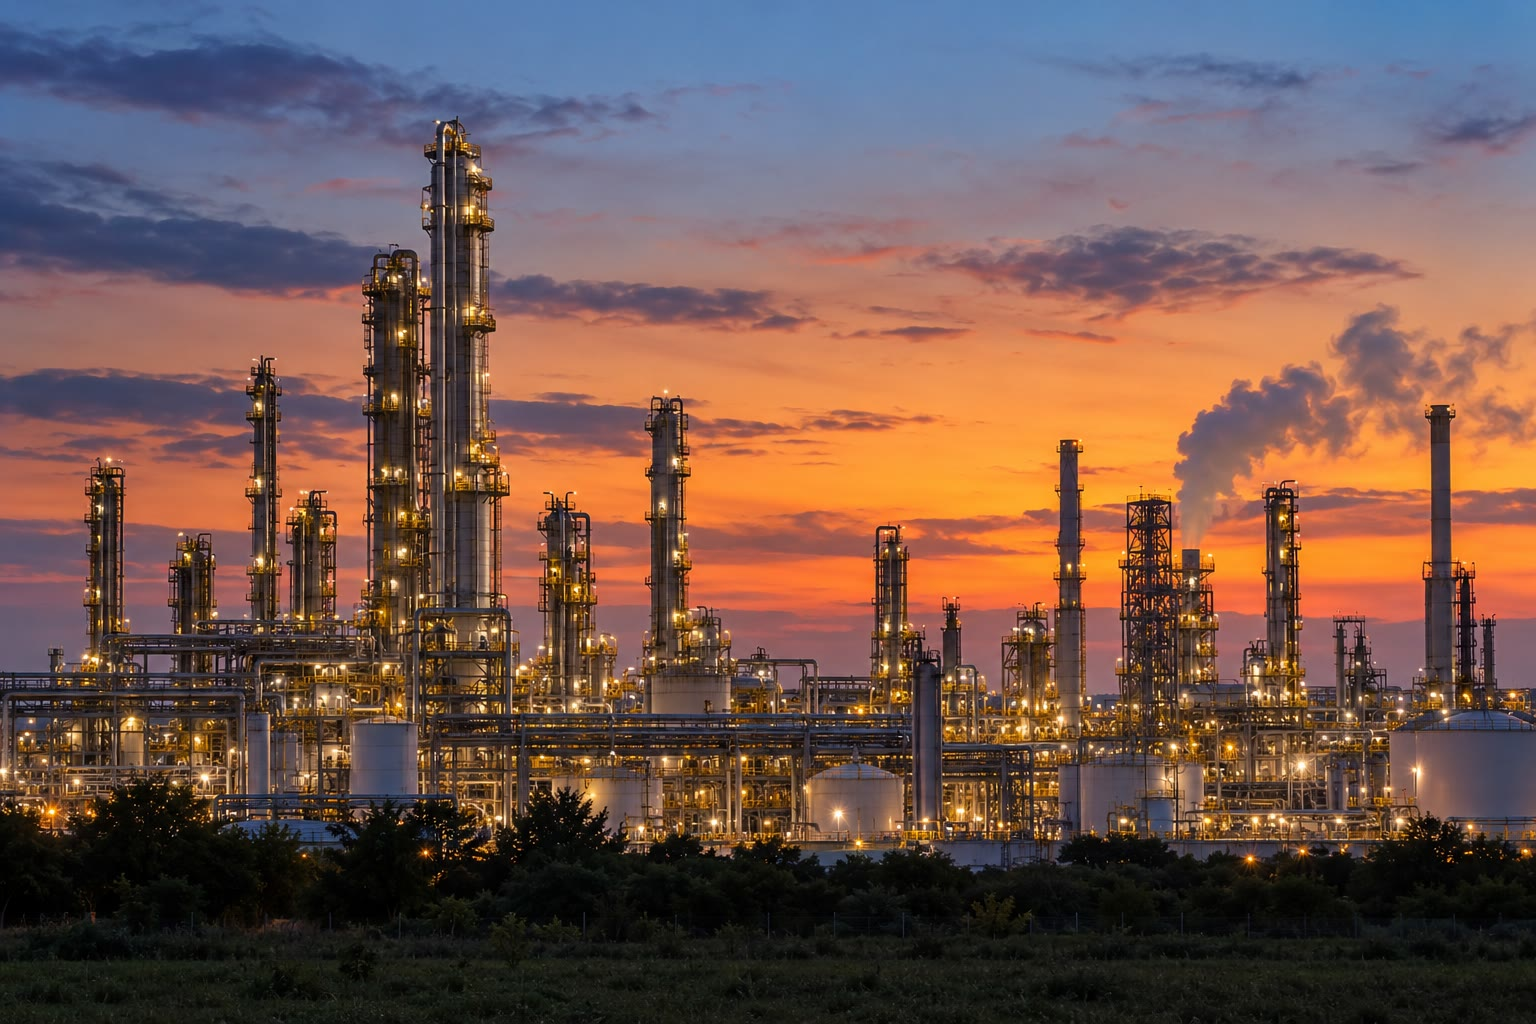
\includegraphics[width=0.6\linewidth]{images/book4/ai/b3-21-chemical-plant.jpg}

{\small संध्या के समय एक बड़ा रासायनिक संयंत्र। \omterm{def:b3:homogeneous-catalysis:carbonylation}{कार्बोनिलन} इकाई में उत्प्रेरक
अभिक्रिया द्रव में घुला एक धातु संकुल होता है; संयंत्र का अधिकांश भाग
पृथक्करण और पुनर्चक्रण करता है।}
\end{omfigure}

\section{हाइड्रोजनन}

\begin{method}[उत्प्रेरकी चक्र पढ़ना]\label{met:b3:homogeneous-catalysis:read-cycle}
\begin{enumerate}
  \item प्रत्येक स्पीशीज़ पर संयोजकता इलेक्ट्रॉन गिनिए और धातु की ऑक्सीकरण
        अवस्था तथा $d^n$ बताइए।
  \item प्रत्येक चरण का नाम बताइए (लिगैंड का निकास या योग, ऑक्सीकारी योग,
        निवेशन, विलोपन) और जाँचिए कि गणनाएँ उसकी अपेक्षा के अनुसार बदलती हैं
        (ऑक्सीकारी योग: ऑक्सीकरण अवस्था और इलेक्ट्रॉन गणना में $+2$)।
  \item विराम अवस्था (संचित होने वाली स्पीशीज़) और
        दर-निर्धारक चरण पहचानिए; दर नियम उनके बीच के पूर्व-साम्यों से
        निकलता है।
\end{enumerate}
\end{method}

\begin{omfigure}
\begin{tikzpicture}[font=\small, >=Stealth]
  \node (a) at (90:2.3) {\ce{RhCl(PPh3)2} \ (14, Rh$^{\mathrm I}$)};
  \node (b) at (0:3.0) {\ce{RhClH2(PPh3)2} \ (16, Rh$^{\mathrm{III}}$)};
  \node (c) at (-90:2.3) {\ce{RhClH2(RCH=CH2)(PPh3)2} \ (18)};
  \node (d) at (180:3.1) {\ce{RhClH(CH2CH2R)(PPh3)2} \ (16)};
  \draw[->, thick] (a) to[bend left=22] node[midway, above right, font=\scriptsize] {$+\,\ce{H2}$, ऑक्सीकारी योग} (b);
  \draw[->, thick] (b) to[bend left=22] node[midway, below right, font=\scriptsize] {$+$ ऐल्कीन} (c);
  \draw[->, thick] (c) to[bend left=22] node[midway, below left, font=\scriptsize] {प्रवासी निवेशन} (d);
  \draw[->, thick] (d) to[bend left=22] node[midway, above left, font=\scriptsize, align=right] {अपचायी\\ विलोपन: $-$ ऐल्केन} (a);
  \node[anchor=south] (p) at (90:3.4) {\ce{RhCl(PPh3)3} \ (16, पूर्व-उत्प्रेरक)};
  \draw[<->, black!50] (p) -- (a) node[midway, right, font=\scriptsize] {$\mp\,\ce{PPh3}$};
\end{tikzpicture}

{\small विल्किन्सन उत्प्रेरक द्वारा ऐल्कीन हाइड्रोजनन का एक सरलीकृत चक्र
(कोष्ठकों में संयोजकता इलेक्ट्रॉन गणनाएँ)। एक फ़ॉस्फ़ीन का निकास एक स्थल खोलता है;
चक्र हाइड्रोजन जोड़ता है, ऐल्कीन को बाँधता है, उसे Rh--H आबंध में निवेशित करता है और
ऐल्केन का विलोपन करता है।}
\end{omfigure}

\begin{proposition}[विल्किन्सन बलगतिकी]\label{prop:b3:homogeneous-catalysis:wilkinson-rate}
यदि $\ce{RhClL3} \rightleftharpoons \ce{RhClL2} + \mathrm L$ ($K_1$) और $\ce{RhClL2} + \ce{H2} \rightleftharpoons \ce{RhClH2L2}$ ($K_2$) तीव्र
साम्य हों और ऐल्कीन के साथ डाइहाइड्राइड की अभिक्रिया (दर स्थिरांक $k$)
दर-निर्धारक हो, तो
\[
  v = \frac{kK_1K_2[\mathrm{Rh}]_{\mathrm{tot}}[\ce{H2}][\text{ऐल्कीन}]}{[\mathrm L] + K_1 + K_1K_2[\ce{H2}]},
\]
जो हाइड्रोजन में संतृप्त होता है और मिलाए गए फ़ॉस्फ़ीन L द्वारा संदमित होता है।
\end{proposition}

\begin{proof}
$[\ce{RhClL2}] = K_1[\ce{RhClL3}]/[\mathrm L]$ और $[\ce{RhClH2L2}] = K_2[\ce{H2}][\ce{RhClL2}]$। $[\mathrm{Rh}]_{\mathrm{tot}}$ को
तीनों स्पीशीज़ के योग के रूप में लिखकर डाइहाइड्राइड के लिए हल करने पर $[\ce{RhClH2L2}] =
K_1K_2[\ce{H2}][\mathrm{Rh}]_{\mathrm{tot}}/([\mathrm L] + K_1 + K_1K_2[\ce{H2}])$ मिलता है; दर $k$ गुणा यह और ऐल्कीन
सांद्रता है।
\end{proof}

विल्किन्सन उत्प्रेरक अबाधित ऐल्कीनों का हाइड्रोजनन प्रतिस्थापित ऐल्कीनों की तुलना में कहीं
तेज़ी से करता है और कार्बोनिल समूहों को अछूता छोड़ देता है: एक
भीड़ भरे धातु केंद्र की वरणात्मकता। किरैल डाइफ़ॉस्फ़ीन इसी रसायन को
असममित हाइड्रोजनन में बदल देते हैं (\cref{ch:b3:asymmetric-synthesis})।

\section{कार्बोनिलन प्रक्रम}

\begin{definition}[हाइड्रोफ़ॉर्मिलन]\label{def:b3:homogeneous-catalysis:hydroformylation}
\emph{हाइड्रोफ़ॉर्मिलन}\index{हाइड्रोफ़ॉर्मिलन} किसी C=C द्विबंध के आर-पार एक हाइड्रोजन परमाणु
और एक फ़ॉर्मिल समूह (CHO) का योग है, $\ce{H2}$ और CO से, जो किसी
ऐल्कीन को एक अधिक कार्बन वाले ऐल्डिहाइड में बदल देता है। \emph{रैखिक-से-शाखित
अनुपात}\index{रैखिक-से-शाखित अनुपात} सीधी-शृंखला
ऐल्डिहाइड और शाखित ऐल्डिहाइड का अनुपात है।
\end{definition}

\emergencystretch=3em पहले प्रक्रमों में $\ce{HCo(CO)4}$ का उपयोग लगभग 150 से \qty{180}{\celsius} पर और अत्यधिक उच्च
दाबों पर होता था। ट्राइफ़ेनिलफ़ॉस्फ़ीन सहित रोडियम लगभग \qty{100}{\celsius} पर और
कहीं कम दाबों पर कार्य करता है, और ऊँचा \omterm{def:b3:homogeneous-catalysis:hydroformylation}{रैखिक-से-शाखित अनुपात} देता है: भारी
फ़ॉस्फ़ीन उस निवेशन का पक्ष लेते हैं जो धातु को अंतस्थ कार्बन पर रखता है।
प्रोपीन ब्यूटेनैल देता है, जिसका हाइड्रोजनन ब्यूटेनॉल में होता है या जिसे सुघट्यकारी
ऐल्कोहॉलों में बदला जाता है।

\begin{definition}[कार्बोनिलन]\label{def:b3:homogeneous-catalysis:carbonylation}
\emph{कार्बोनिलन}\index{कार्बोनिलन} कार्बन मोनोऑक्साइड के साथ अभिक्रिया द्वारा किसी अणु में
कार्बोनिल समूह का प्रवेश है, जो किसी धातु संकुल द्वारा
CO के प्रवासी निवेशन के माध्यम से उत्प्रेरित होता है।
\end{definition}

मेथेनॉल का ऐसीटिक अम्ल में \omterm{def:b3:homogeneous-catalysis:carbonylation}{कार्बोनिलन}, $\ce{CH3OH + CO -> CH3COOH}$, मेथिल आयोडाइड को
सह-उत्प्रेरक के रूप में लेकर रोडियम (मॉनसैंटो प्रक्रम) या इरिडियम (कैटिवा प्रक्रम) पर चलता है:
हाइड्रोजन आयोडाइड मेथेनॉल को मेथिल आयोडाइड में बदलता है, धातु
मेथिल समूह में CO निवेशित करती है, और बना ऐसीटिल आयोडाइड जल-अपघटित होकर
पुनः HI मुक्त करता है।

\begin{omfigure}
\begin{tikzpicture}[font=\small, >=Stealth]
  \node (a) at (90:2.1) {$\ce{[M(CO)2I2]-}$ (16)};
  \node (b) at (0:2.9) {$\ce{[CH3M(CO)2I3]-}$ (18)};
  \node (c) at (-90:2.1) {$\ce{[CH3COM(CO)I3]-}$ (16)};
  \node (d) at (180:2.9) {$\ce{[CH3COM(CO)2I3]-}$ (18)};
  \draw[->, thick] (a) to[bend left=22] node[midway, above right, font=\scriptsize, align=left] {$+\,\ce{CH3I}$\\ ऑक्सीकारी योग} (b);
  \draw[->, thick] (b) to[bend left=22] node[midway, below right, font=\scriptsize] {प्रवासी निवेशन} (c);
  \draw[->, thick] (c) to[bend left=22] node[midway, below left, font=\scriptsize] {$+$ CO} (d);
  \draw[->, thick] (d) to[bend left=22] node[midway, above left, font=\scriptsize, align=right] {अपचायी विलोपन\\ $-\,\ce{CH3COI}$} (a);
  \node[anchor=north, align=center, font=\scriptsize] at (0,-2.55) {$\ce{CH3COI + H2O -> CH3COOH + HI}$, \quad $\ce{CH3OH + HI -> CH3I + H2O}$};
\end{tikzpicture}

{\small $\mathrm M = \mathrm{Rh}$ के लिए मेथेनॉल का \omterm{def:b3:homogeneous-catalysis:carbonylation}{कार्बोनिलन} चक्र (मॉनसैंटो); कोष्ठकों में संयोजकता
इलेक्ट्रॉन गणनाएँ, धातु की ऑक्सीकरण अवस्था ऊपर I, अन्यत्र III।
रोडियम के साथ मेथिल आयोडाइड का ऑक्सीकारी योग दर-निर्धारक है।
इरिडियम (कैटिवा) के साथ यह कहीं तेज़ है, प्रवासी निवेशन धीमा है, और
\omterm{def:b3:surfaces-catalysis:catalyst-design}{वर्धक}, जो $\ce{[CH3Ir(CO)2I3]-}$ से एक आयोडाइड हटाते हैं, निवेशन को तेज़ करते हैं।}
\end{omfigure}

\begin{proposition}[रोडियम प्रक्रम का दर नियम]\label{prop:b3:homogeneous-catalysis:monsanto-rate}
यदि $\ce{[Rh(CO)2I2]-}$ में मेथिल आयोडाइड का ऑक्सीकारी योग दर-निर्धारक हो और
यह संकुल विराम अवस्था हो, तो $v = k[\mathrm{Rh}]_{\mathrm{tot}}[\ce{CH3I}]$: CO में और
मेथेनॉल में शून्य कोटि।
\end{proposition}

\begin{proof}
दर धीमे चरण की दर है, $k[\ce{[Rh(CO)2I2]-}][\ce{CH3I}]$, और लगभग सारा रोडियम
विराम अवस्था में है। CO केवल धीमे चरण के बाद प्रवेश करता है, और मेथेनॉल केवल
मेथिल आयोडाइड को पुनर्जनित करता है, जिसकी स्थायी सांद्रता मेथेनॉल के बजाय
रिएक्टर में डाले गए आयोडाइड से तय होती है।
\end{proof}

नए संयंत्रों में व्यावहारिक कारणों से इरिडियम रोडियम पर भारी पड़ा: इसके संकुल
कम जल सांद्रता पर भी विलयन में बने रहते हैं, जिससे उत्पाद को सुखाने में ऊर्जा
बचती है, और वे कम उप-उत्पाद देते हैं। दोनों की मुख्य पार्श्व अभिक्रिया
जल--गैस विस्थापन है, $\ce{CO + H2O -> CO2 + H2}$, जो उसी धातु द्वारा उत्प्रेरित होती है और
कार्बन मोनोऑक्साइड को व्यर्थ करती है।

\section{ओलेफ़िन मेटाथीसिस}

\begin{definition}[ओलेफ़िन मेटाथीसिस]\label{def:b3:homogeneous-catalysis:metathesis}
\emph{ओलेफ़िन मेटाथीसिस}\index{ओलेफ़िन मेटाथीसिस} दो ऐल्कीनों के
ऐल्किलिडीन अर्धों का विनिमय है, $\mathrm{RCH{=}CHR + R'CH{=}CHR' \rightleftharpoons 2\,RCH{=}CHR'}$, जो
धातु \omterm{def:b3:organometallic-bonding:carbene}{कार्बीन संकुलों} द्वारा एक \emph{धातुसाइक्लोब्यूटेन}\index{धातुसाइक्लोब्यूटेन} के माध्यम से उत्प्रेरित होता है,
जो धातु और तीन कार्बनों का एक चतुःसदस्यीय वलय है। इसके संश्लेषी रूप हैं
\emph{वलय-समापी मेटाथीसिस}\index{वलय-समापी मेटाथीसिस} (RCM), जो
एक अणु के दो ऐल्कीन सिरों को एथीन के निकास के साथ एक वलय में जोड़ता है,
तनावग्रस्त चक्रीय ऐल्कीनों का \emph{वलय-विवृत मेटाथीसिस बहुलकीकरण}\index{वलय-विवृत मेटाथीसिस बहुलकीकरण}
(ROMP), और दो भिन्न ऐल्कीनों के बीच \emph{संकर
मेटाथीसिस}\index{संकर मेटाथीसिस}।
\end{definition}

\begin{definition}[शोवें क्रियाविधि]\label{def:b3:homogeneous-catalysis:chauvin}
मेटाथीसिस की \emph{शोवें क्रियाविधि}\index{शोवें क्रियाविधि} किसी ऐल्कीन का $[2+2]$ चक्रीयोजन है,
किसी धातु \omterm{def:b3:organometallic-bonding:carbene}{कार्बीन}, $\mathrm{[M]{=}CHR}$, पर, जिससे एक
\omterm{def:b3:homogeneous-catalysis:metathesis}{धातुसाइक्लोब्यूटेन} बनता है, और उसके बाद दूसरी दिशा में उसका चक्र-प्रत्यावर्तन,
जो एक नया ऐल्कीन और एक नई \omterm{def:b3:organometallic-bonding:carbene}{कार्बीन} मुक्त करता है।
\end{definition}

\begin{omfigure}
\setchemfig{atom sep=2.1em}
\schemestart
\chemfig{M=[:0]CHR}
\+
\chemfig{R'HC=[:0]CHR'}
\arrow{<=>}
\chemfig{M?-[:0]CHR-[:-90]CHR'-[:180]CHR'?}
\arrow{<=>}
\chemfig{M=[:0]CHR'}
\+
\chemfig{RHC=[:0]CHR'}
\schemestop
\par\vspace{10pt}

{\small \omterm{def:b3:homogeneous-catalysis:chauvin}{शोवें क्रियाविधि}: एक धातु \omterm{def:b3:organometallic-bonding:carbene}{कार्बीन} और एक ऐल्कीन मिलकर एक
\omterm{def:b3:homogeneous-catalysis:metathesis}{धातुसाइक्लोब्यूटेन} बनाते हैं, जो दूसरी ओर से खुलकर एक नई \omterm{def:b3:organometallic-bonding:carbene}{कार्बीन} और एक नया
ऐल्कीन देता है। प्रत्येक चरण उत्क्रमणीय है: मेटाथीसिस साम्य तक पहुँचता है, जब तक कि कोई
उत्पाद निकल न जाए।}
\end{omfigure}

\begin{proposition}[वलय-समापी मेटाथीसिस को आगे बढ़ाना]\label{prop:b3:homogeneous-catalysis:metathesis-equilibrium}
वलय समापन $\text{डाईन} \rightleftharpoons \text{साइक्लोऐल्कीन} + \ce{C2H4}$ के लिए, विलयन से एथीन हटाने पर
अभिक्रिया पूर्णता तक जाती है; गैस अणु के मुक्त होने की एन्ट्रॉपी
अभिक्रिया का पक्ष लेती है।
\end{proposition}

\begin{proof}
साम्य पर $K = [\text{वलय}][\ce{C2H4}]/[\text{डाईन}]$: यदि शोधन या
निर्वातन द्वारा $[\ce{C2H4}]$ कम रखा जाए, तो $[\text{वलय}]/[\text{डाईन}] = K/[\ce{C2H4}]$ असीमित रूप से बढ़ता है। अभिक्रिया में
अणुओं की संख्या एक बढ़ती है, जबकि बने और टूटे आबंध (प्रत्येक एक C=C)
समान हैं: तनावरहित वलय के लिए $\Delta_rH^\circ \approx 0$ और $\Delta_rS^\circ > 0$, अतः $K$ अनुकूल है।
\end{proof}

नॉरबोर्नीन जैसे तनावग्रस्त वलयों का ROMP विपरीत कारण से दूसरी दिशा में चलता है:
वलय तनाव का मोचन स्थानांतरीय एन्ट्रॉपी की हानि की भरपाई करता है।
रॉबर्ट ग्रब्स की रूथेनियम \omterm{def:b3:organometallic-bonding:carbene}{कार्बीनें} जल, वायु और अधिकांश क्रियात्मक
समूहों को सहन करती हैं; रिचर्ड श्रॉक की मॉलिब्डेनम और टंगस्टन ऐल्किलिडीनें अधिक सक्रिय हैं
और प्रतिबिंबवरणात्मक बनाई जा सकती हैं।

\section{पैलेडियम क्रॉस-युग्मन}

\begin{definition}[क्रॉस-युग्मन अभिक्रियाएँ]\label{def:b3:homogeneous-catalysis:cross-coupling}
\emph{क्रॉस-युग्मन अभिक्रिया}\index{क्रॉस-युग्मन अभिक्रिया} दो
भिन्न कार्बन अणुखंडों, एक कार्बनिक हैलाइड और एक कार्बधात्विक अभिकर्मक या एक
ऐल्कीन, को किसी धातु उत्प्रेरक, प्रायः पैलेडियम, पर जोड़ती है। \emph{हेक
अभिक्रिया}\index{हेक अभिक्रिया} में एक ऐरिल या वाइनिल हैलाइड किसी ऐल्कीन से युग्मित होकर
एक प्रतिस्थापित ऐल्कीन देता है; \emph{सुज़ुकी--मियाउरा
युग्मन}\index{सुज़ुकी--मियाउरा युग्मन} में यह किसी क्षारक की उपस्थिति में एक कार्बबोरॉन
यौगिक से युग्मित होता है।
\end{definition}

\begin{omfigure}
\begin{tikzpicture}[font=\small, >=Stealth]
  \node (a) at (90:2.0) {$\mathrm{Pd^0L_2}$};
  \node (b) at (0:2.6) {$\mathrm{ArPd^{II}XL_2}$};
  \node (c) at (-90:2.0) {$\mathrm{ArPd^{II}Ar'L_2}$};
  \draw[->, thick] (a) to[bend left=25] node[midway, above right, font=\scriptsize, align=left] {$+\,$ArX\\ ऑक्सीकारी योग} (b);
  \draw[->, thick] (b) to[bend left=25] node[midway, below right, font=\scriptsize, align=left] {$+\,\mathrm{Ar'B(OH)_2}$, क्षारक\\ पारधात्वन} (c);
  \draw[->, thick] (c) to[bend left=35] node[midway, left, font=\scriptsize, align=right] {अपचायी विलोपन\\ $-\,$Ar--Ar$'$} (a);
\end{tikzpicture}

{\small सुज़ुकी--मियाउरा चक्र: पैलेडियम(0) ऐरिल हैलाइड के C--X आबंध में
निवेशित होता है, क्षारक द्वारा सक्रियित बोरोनिक अम्ल से दूसरा ऐरिल समूह
ग्रहण करता है, और अपचायी विलोपन द्वारा बाइऐरिल मुक्त करता है।}
\end{omfigure}

\begin{method}[क्रॉस-युग्मन का चयन]\label{met:b3:homogeneous-catalysis:choose-coupling}
\begin{enumerate}
  \item लक्ष्य को बनाए जाने वाले C--C आबंध पर विच्छेदित कीजिए; एक साथी
        हैलाइड बनता है (अभिक्रियाशीलता में आयोडाइड $>$ ब्रोमाइड $>$ ट्राइफ़्लेट $>$ क्लोराइड), दूसरा
        बोरोनिक अम्ल (सुज़ुकी--मियाउरा), ऐल्कीन (हेक), कार्बज़िंक
        (नेगीशी) या कॉपर(I) सहित अंतस्थ ऐल्काइन (सोनोगाशिरा)।
  \item ऐसे साथी-युग्म को वरीयता दीजिए जिसके अभिकर्मक स्थायी, उपलब्ध और सबसे कम
        विषैले हों: बाइऐरिलों के लिए बोरोनिक अम्ल।
  \item सबसे कठिन चरण के लिए लिगैंड चुनिए: इलेक्ट्रॉन-समृद्ध, भारी फ़ॉस्फ़ीन
        या \omterm{def:b3:organometallic-bonding:carbene}{N-विषमचक्रीय कार्बीनें} क्लोराइडों के ऑक्सीकारी योग को तेज़ करती हैं।
  \item उत्पाद से पैलेडियम को औषधों में अनुमत निम्न स्तरों तक हटाने की योजना
        बनाइए (अपमार्जक रेज़िन, क्रिस्टलन)।
\end{enumerate}
\end{method}

\section{बहुलकीकरण उत्प्रेरण}

\begin{definition}[ज़ीग्लर--नाटा उत्प्रेरण]\label{def:b3:homogeneous-catalysis:ziegler-natta}
\emph{ज़ीग्लर--नाटा उत्प्रेरक}\index{ज़ीग्लर--नाटा उत्प्रेरक} निम्न दाब पर
ऐल्कीनों का बहुलकीकरण करता है; यह किसी संक्रमण-धातु हैलाइड, प्रायः
टाइटेनियम के, और एक ऐल्किलऐलुमिनियम यौगिक से बनता है। शृंखला वृद्धि की \emph{कोसी--आर्लमैन
क्रियाविधि}\index{कोसी--आर्लमैन क्रियाविधि} धातु पर बढ़ती ऐल्किल शृंखला के सिस
स्थित किसी रिक्त स्थल पर ऐल्कीन का उपसहसंयोजन है,
जिसके बाद धातु--कार्बन आबंध में उसका प्रवासी निवेशन होता है, जो फिर से एक
रिक्त स्थल छोड़ता है। \emph{एकल-स्थल उत्प्रेरक}\index{एकल-स्थल उत्प्रेरक} के
सभी सक्रिय केंद्र सर्वसम होते हैं, जैसे किसी आण्विक \omterm{def:b3:organometallic-bonding:metallocene}{मेटैलोसीन} उत्प्रेरक में।
\end{definition}

\begin{omfigure}
\begin{tikzpicture}[font=\small, >=Stealth]
  \begin{scope}[every node/.style={inner sep=1pt}]
  % panel 1: chain and vacant site
  \node (m1) at (0,0) {M};
  \node (p1) at (-0.7,0.55) {P};
  \node (v1) at (0.7,0.55) {$\square$};
  \draw (m1) -- (p1);
  % panel 2: alkene bound side-on at the vacant site
  \node (m2) at (3.6,0) {M};
  \node (p2) at (2.9,0.55) {P};
  \node (c2a) at (4.75,1.25) {\ce{CH2}};
  \node (c2b) at (4.75,0.25) {\ce{CH2}};
  \draw (m2) -- (p2);
  \draw[double, double distance=1.6pt] (c2a) -- (c2b);
  \draw[dashed] (m2) -- (4.55,0.75);
  % panel 3: chain longer by two carbons, vacant site moved
  \node (m3) at (7.7,0) {M};
  \node (v3) at (7.0,0.55) {$\square$};
  \node (c3a) at (8.45,0.55) {\ce{CH2}};
  \node (c3b) at (8.45,1.45) {\ce{CH2}};
  \node (p3) at (7.75,1.95) {P};
  \draw (m3) -- (c3a) -- (c3b) -- (p3);
  \end{scope}
  \draw[->, thick] (1.25,0.35) -- (2.55,0.35) node[midway, above, font=\scriptsize] {$+\,\ce{C2H4}$};
  \draw[->, thick] (5.35,0.35) -- (6.3,0.35) node[midway, above, font=\scriptsize] {निवेशन};
\end{tikzpicture}
\par\medskip

{\small \omterm{def:b3:homogeneous-catalysis:ziegler-natta}{कोसी--आर्लमैन क्रियाविधि} (P: बढ़ती बहुलक शृंखला; $\square$: एक
रिक्त स्थल)। ऐल्कीन शृंखला के बगल में बँधता है और एक चतुःसदस्यीय संक्रमण अवस्था
से होकर M--C आबंध में निवेशित होता है; शृंखला, जो दो
कार्बन लंबी हो गई है, अब उस स्थल पर है जहाँ ऐल्कीन था, और रिक्त स्थल
खिसक गया है।}
\end{omfigure}

\begin{proposition}[उत्प्रेरक सममिति से टैक्टिसिटी]\label{prop:b3:homogeneous-catalysis:tacticity-symmetry}
ऐसे \omterm{def:b3:organometallic-bonding:metallocene}{मेटैलोसीन} उत्प्रेरक के लिए जिस पर शृंखला प्रत्येक निवेशन पर दो उपसहसंयोजन
स्थलों के बीच प्रवास करती है, $C_2$-सममित उत्प्रेरक आइसोटैक्टिक
पॉलिप्रोपिलीन देता है और $C_s$-सममित उत्प्रेरक सिंडियोटैक्टिक पॉलिप्रोपिलीन।
\end{proposition}

\begin{proof}[तर्क]
निवेशित होने वाले प्रोपीन का फलक स्थल के किरैल परिवेश द्वारा चुना जाता है।
$C_2$-सममित उत्प्रेरक में दोनों स्थल $C_2$ अक्ष द्वारा परस्पर बदले जाते हैं,
जो हस्तता को संरक्षित रखता है (\cref{ch:b3:point-groups}): दोनों स्थल
एक ही फलक चुनते हैं, और क्रमागत मेथिल समूहों का विन्यास समान होता है (आइसोटैक्टिक)।
$C_s$-सममित उत्प्रेरक में दोनों स्थल दर्पण प्रतिबिंब हैं: वे विपरीत
फलक चुनते हैं, और विन्यास एकांतर होते हैं (सिंडियोटैक्टिक)। जिस उत्प्रेरक के स्थल
अकिरैल हों, जैसे मेथिलऐलुमिनॉक्सेन के साथ असेतुबद्ध $\ce{Cp2ZrCl2}$, वह ऐटैक्टिक
बहुलक देता है।
\end{proof}

\begin{proposition}[शुल्ज़--फ़्लोरी वितरण]\label{prop:b3:homogeneous-catalysis:schulz-flory}
यदि \omterm{def:b3:homogeneous-catalysis:ziegler-natta}{एकल-स्थल उत्प्रेरक} पर प्रत्येक बढ़ती शृंखला नियत
प्रायिकता $p$ के साथ एक एकलक जोड़ती है और अन्यथा स्थानांतरित (समाप्त) होती है, तो
$n$ इकाइयों वाली शृंखलाओं का संख्या अंश $x_n = (1 - p)p^{n-1}$ है, और परिक्षेपिता $M_w/M_n = 1 + p$ लंबी शृंखलाओं के लिए 2 की ओर प्रवृत्त होती है।
\end{proposition}

\begin{proof}
ठीक $n$ इकाइयों वाली शृंखला $n - 1$ बार बढ़ी है और एक बार रुकी है:
प्रायिकता $p^{n-1}(1 - p)$। तब $\sum nx_n = 1/(1 - p)$ (संख्या औसत), और द्रव्यमान
अंश $w_n = nx_n(1 - p)$ द्रव्यमान औसत $\sum nw_n = (1 + p)/(1 - p)$ देते हैं। उनका
अनुपात $1 + p$ है।
\end{proof}

\begin{omfigure}
\begin{tikzpicture}
\begin{axis}[width=0.7\linewidth, height=5.2cm, xmin=0, xmax=200, ymin=0, ymax=1.05,
  axis lines=left, xlabel={$M$ / \unit{kg.mol^{-1}}}, ylabel={प्रति इकाई अंश (मापित)},
  tick label style={font=\small}, label style={font=\small},
  legend style={font=\scriptsize, draw=none, at={(0.98,0.98)}, anchor=north east}, legend cell align=left]
\addplot[omDef, line width=1pt] table[x=M_kg, y=x] {figdata/out/bachelor-3-schulz-flory.dat};
\addplot[omThm, line width=1pt] table[x=M_kg, y expr=\thisrow{w}/0.368] {figdata/out/bachelor-3-schulz-flory.dat};
\draw[black!40, dashed] (axis cs:28.05,0) -- (axis cs:28.05,1);
\node[font=\scriptsize, anchor=west] at (axis cs:30,0.5) {$M_n$};
\legend{संख्या अंश, द्रव्यमान अंश (अपने अधिकतम पर मापित)}
\end{axis}
\end{tikzpicture}

{\small \omterm{def:b3:homogeneous-catalysis:ziegler-natta}{एकल-स्थल उत्प्रेरक} पर बने पॉलिएथिलीन का सर्वाधिक प्रायिक मोलर-द्रव्यमान वितरण
(मॉडल: माध्य बहुलकीकरण की कोटि 1000): संख्या
अंश चरघातांकी रूप से गिरता है, द्रव्यमान अंश $M_n \approx \qty{28}{kg/mol}$ पर शिखर बनाता है; $M_w = 2M_n$। पारंपरिक
\omterm{def:b3:homogeneous-catalysis:ziegler-natta}{ज़ीग्लर--नाटा उत्प्रेरक}, अनेक प्रकार के स्थलों के साथ, अधिक चौड़े
वितरण देते हैं।}
\end{omfigure}

\begin{inthelab}[एक सुज़ुकी युग्मन और उसका पैलेडियम]
ऐरिल ब्रोमाइड, बोरोनिक अम्ल (1.2 तुल्यांक), पोटैशियम कार्बोनेट और
एक पैलेडियम फ़ॉस्फ़ीन संकुल के प्रतिशत के कुछ दशांश को नाइट्रोजन के अधीन टॉलूईन, एथेनॉल और जल के एक
विगैसित मिश्रण में पश्चवाह पर विलोडित किया जाता है। कार्य-समापन के बाद
अपरिष्कृत बाइऐरिल को पैलेडियम बाँधने वाली थायोल-क्रियात्मकीकृत सिलिका के साथ विलोडित किया जाता है,
छाना जाता है और क्रिस्टलित किया जाता है; बचे हुए पैलेडियम को
प्लाज़्मा द्रव्यमान स्पेक्ट्रममिति से मापा जाता है।
\end{inthelab}

\begin{safety}{\ghs[0.62cm]{GHS02}\ghs[0.62cm]{GHS04}\ghs[0.62cm]{GHS06}\ghs[0.62cm]{GHS08}}
% ledger: ghs4:MeI, ghs:CO
मेथिल आयोडाइड: साँस द्वारा लेने और निगलने पर विषैला, त्वचा के संपर्क में हानिकारक, संदिग्ध
कैंसरजन, वाष्पशील; धूम-हुड में सँभाला जाता है। कार्बन मोनोऑक्साइड: अत्यधिक
ज्वलनशील, साँस द्वारा लेने पर विषैला, अजन्मे शिशु को क्षति पहुँचा सकता है, गंधहीन;
स्थायी संसूचकों और अलार्मों के साथ प्रयुक्त।
\end{safety}

\begin{history}[ज़ीग्लर, नाटा, और मेटाथीसिस]
कार्ल ज़ीग्लर ने 1953 में पाया कि टाइटेनियम क्लोराइड और ऐल्किलऐलुमिनियम यौगिक
वायुमंडलीय दाब पर एथीन का बहुलकीकरण करते हैं, और जूलियो नाटा ने 1954 में कि ऐसे
उत्प्रेरक त्रिविम-नियमित पॉलिप्रोपिलीन बनाते हैं; उन्होंने रसायन का 1963 का नोबेल पुरस्कार
साझा किया। ईव शोवें ने 1971 में मेटाथीसिस की \omterm{def:b3:homogeneous-catalysis:metathesis}{धातुसाइक्लोब्यूटेन} क्रियाविधि
प्रस्तावित की; रॉबर्ट ग्रब्स और रिचर्ड श्रॉक के साथ, जिन्होंने सुपरिभाषित
मेटाथीसिस उत्प्रेरक बनाए, उन्हें रसायन का 2005 का नोबेल पुरस्कार मिला।
\end{history}

\section{अभ्यास}

\begin{exercise}[$\star$]\label{exo:b3:homogeneous-catalysis:1}
चित्र के विल्किन्सन चक्र के प्रत्येक चरण पर रोडियम की संयोजकता इलेक्ट्रॉन गणना और
ऑक्सीकरण अवस्था बताइए।
\end{exercise}

\begin{exercise}[$\star$]\label{exo:b3:homogeneous-catalysis:2}
प्रोपीन के \omterm{def:b3:homogeneous-catalysis:hydroformylation}{हाइड्रोफ़ॉर्मिलन} से बनने वाले दोनों ऐल्डिहाइडों के नाम बताइए। कौन-सा
रैखिक है?
\end{exercise}

\begin{exercise}[$\star$]\label{exo:b3:homogeneous-catalysis:3}
डाइएथिल डाइऐलिलमैलोनेट, $\ce{(CH2=CHCH2)2C(CO2Et)2}$, \omterm{def:b3:homogeneous-catalysis:metathesis}{वलय-समापी मेटाथीसिस} से गुज़रता है।
उत्पाद और उसके वलय का आकार बताइए।
\end{exercise}

\begin{exercise}[$\star$]\label{exo:b3:homogeneous-catalysis:4}
मेथिल ऐक्रिलेट के साथ आयोडोबेंज़ीन की \omterm{def:b3:homogeneous-catalysis:cross-coupling}{हेक अभिक्रिया} का उत्पाद, और उसका
विन्यास बताइए।
\end{exercise}

\begin{exercise}[$\star\star$]\label{exo:b3:homogeneous-catalysis:5}
रोडियम प्रक्रम के चक्र से आरंभ करके उसका दर नियम व्युत्पन्न कीजिए, और समझाइए
कि मेथेनॉल का रूपांतरण लगभग पूर्ण होने तक दर को क्यों नहीं बदलता।
\end{exercise}

\begin{exercise}[$\star\star$]\label{exo:b3:homogeneous-catalysis:6}
4-मेथिलबाइफ़ेनिल के दो सुज़ुकी--मियाउरा विच्छेदन प्रस्तावित कीजिए और एक चुनिए।
\end{exercise}

\begin{exercise}[$\star\star$]\label{exo:b3:homogeneous-catalysis:7}
$C_2$-सममित सेतुबद्ध
बिस(इंडेनिल)ज़र्कोनियम उत्प्रेरक, एक $C_s$-सममित उत्प्रेरक, और असेतुबद्ध $\ce{Cp2ZrCl2}$ से बने पॉलिप्रोपिलीन की टैक्टिसिटी का पूर्वानुमान कीजिए।
\end{exercise}

\begin{exercise}[$\star\star$]\label{exo:b3:homogeneous-catalysis:8}
\qty{0.10}{mol\%} उत्प्रेरक के साथ एक हाइड्रोजनन \qty{2.0}{h} में 98\,\% रूपांतरण तक पहुँचता है।
आवर्त संख्या और माध्य आवर्त आवृत्ति परिकलित कीजिए।
\end{exercise}

\begin{exercise}[$\star\star$]\label{exo:b3:homogeneous-catalysis:9}
नॉरबोर्नीन के वलय-विवृत मेटाथीसिस से बने बहुलक की पुनरावृत्त इकाई बनाइए,
और समझाइए कि अभिक्रिया पूर्णता तक क्यों जाती है।
\end{exercise}

\begin{exercise}[$\star\star\star$]\label{exo:b3:homogeneous-catalysis:10}
एक \omterm{def:b3:homogeneous-catalysis:ziegler-natta}{एकल-स्थल उत्प्रेरक} $p = 0.9995$ वाली शृंखलाएँ देता है। संख्या-औसत
बहुलकीकरण की कोटि और परिक्षेपिता परिकलित कीजिए। ज़ीग्लर--नाटा बहुलक
अधिक चौड़ा क्यों होता है?
\end{exercise}

\begin{exercise}[$\star\star\star$]\label{exo:b3:homogeneous-catalysis:11}
विल्किन्सन दर नियम से दिखाइए कि निम्न दाब पर दर $\ce{H2}$ में प्रथम कोटि की है
और उच्च दाब पर उससे स्वतंत्र, तथा फ़ॉस्फ़ीन मिलाने से
अभिक्रिया धीमी होती है।
\end{exercise}

\begin{exercise}[$\star\star\star$]\label{exo:b3:homogeneous-catalysis:12}
समझाइए कि रोडियम \omterm{def:b3:homogeneous-catalysis:hydroformylation}{हाइड्रोफ़ॉर्मिलन} में भारी फ़ॉस्फ़ीन \omterm{def:b3:homogeneous-catalysis:hydroformylation}{रैखिक-से-शाखित अनुपात} क्यों बढ़ाते हैं,
और ऐल्डिहाइडों से बनने वाले सुघट्यकारी ऐल्कोहॉलों के लिए ऊँचा अनुपात
क्यों महत्त्वपूर्ण है।
\end{exercise}

\section{समस्या: मेथेनॉल से सिरके तक}

\begin{problem}[{सप्ताहांत समस्या --- इरिडियम चक्र पर मेथेनॉल से सिरके तक:
चक्र की गणनाएँ और चरण, उसका दर-निर्धारक चरण और वर्धक, एक
संयंत्र की आवर्त आवृत्ति, और जल--गैस विस्थापन में व्यर्थ हुई
कार्बन मोनोऑक्साइड}]
\label{pb:b3:homogeneous-catalysis:1}
% ledger: aw:Ir, aw:C, aw:H, aw:O
एक ऐसीटिक अम्ल संयंत्र (समस्या के आँकड़े) प्रति वर्ष $\qty{5.0e5}{t}$ ऐसीटिक अम्ल
\qty{8000}{h} के प्रचालन में बनाता है, \qty{200}{m^3} अभिक्रिया द्रव के साथ जिसमें \qty{5.0}{mmol/L}
इरिडियम है। कार्बन मोनोऑक्साइड पर इसकी वरणात्मकता 94\,\% है: शेष
जल--गैस विस्थापन द्वारा रूपांतरित होता है।

\medskip\noindent\textbf{भाग I --- चक्र।}
\begin{enumerate}
  \item $\ce{[Ir(CO)2I2]-}$ के इलेक्ट्रॉन गिनिए और उसकी ऑक्सीकरण अवस्था बताइए।
  \item $\ce{CH3I}$ का ऑक्सीकारी योग: उत्पाद, गणना, ऑक्सीकरण अवस्था?
  \item आयोडाइड का निकास और CO का योग: कौन-सा उदासीन संकुल बनता है?
  \item प्रवासी निवेशन: उत्पाद और गणना?
  \item आयोडाइड का योग, फिर ऐसीटिल आयोडाइड का अपचायी विलोपन: क्या
        पुनर्जनित होता है?
  \item जल और मेथेनॉल के साथ चक्र को पूरा करने वाले दो कार्बनिक चरण लिखिए।
  \item समग्र अभिक्रिया लिखिए।
\end{enumerate}

\medskip\noindent\textbf{भाग II --- बलगतिकी।}
\begin{enumerate}[resume]
  \item इरिडियम के साथ कौन-सा चरण दर-निर्धारक है, और यह रोडियम से
        कैसे भिन्न है?
  \item आयोडाइड को पकड़ने वाले \omterm{def:b3:surfaces-catalysis:catalyst-design}{वर्धक} चक्र को कैसे त्वरित करते हैं?
  \item यह आयोडाइड सांद्रता पर किस निर्भरता का पूर्वानुमान करता है?
  \item दर मेथेनॉल सांद्रता से स्वतंत्र क्यों है?
\end{enumerate}

\medskip\noindent\textbf{भाग III --- संयंत्र।}
\begin{enumerate}[resume]
  \item प्रति वर्ष बने ऐसीटिक अम्ल की मात्रा परिकलित कीजिए।
  \item प्रति घंटे मात्रा परिकलित कीजिए।
  \item रिएक्टर में इरिडियम की मात्रा, और उसका द्रव्यमान, परिकलित कीजिए।
  \item आवर्त आवृत्ति परिकलित कीजिए।
  \item प्रति वर्ष आवर्त संख्या परिकलित कीजिए।
  \item दिक्--काल लब्धि किलोग्राम प्रति घन मीटर प्रति घंटे में परिकलित कीजिए।
\end{enumerate}

\medskip\noindent\textbf{भाग IV --- जल--गैस विस्थापन।}
\begin{enumerate}[resume]
  \item जल--गैस विस्थापन अभिक्रिया लिखिए।
  \item प्रति मोल ऐसीटिक अम्ल उपभुक्त CO परिकलित कीजिए।
  \item प्रति मोल ऐसीटिक अम्ल बनी \ce{CO2} परिकलित कीजिए।
  \item प्रति टन ऐसीटिक अम्ल उत्सर्जित \ce{CO2} का द्रव्यमान परिकलित कीजिए।
  \item निम्नतर जल सांद्रता पर प्रचालन क्यों सहायक है, और इसे क्या सीमित करता है?
  \item विस्थापन और कौन-सा उत्पाद बनाता है, और रिएक्टर में यह समस्या
        क्यों है?
  \item परिणाम बताइए: इरिडियम उत्प्रेरक की आवर्त आवृत्ति।
\end{enumerate}
\end{problem}
